% !TEX program = xelatex
\documentclass[UTF8,a4paper,11pt]{ctexart}

\usepackage[left=2.35cm,right=2.35cm,top=2.25cm,bottom=2.35cm]{geometry}
\usepackage{amsmath,amssymb,mathtools,bm}
\usepackage{booktabs,tabularx,array,multirow}
\usepackage{graphicx,grffile}
\usepackage{xcolor}
\usepackage{hyperref}
\usepackage{enumitem}
\usepackage{titlesec}
\usepackage{fancyhdr}
\usepackage{caption}
\usepackage{float}
\usepackage{microtype}

\definecolor{navy}{HTML}{16324F}
\definecolor{teal}{HTML}{007F82}
\definecolor{softgray}{HTML}{F2F5F7}
\definecolor{rulegray}{HTML}{CFD8DC}
\hypersetup{colorlinks=true,linkcolor=navy,urlcolor=teal,citecolor=navy,pdftitle={ROCA-HiWA},pdfauthor={OT-HiWA Project}}
\setlength{\parskip}{0.45em}
\setlength{\parindent}{2em}
\setlength{\headheight}{22pt}
\setlength{\emergencystretch}{2em}
\renewcommand{\arraystretch}{1.22}
\setlist[itemize]{leftmargin=1.8em,itemsep=0.25em,topsep=0.25em}
\setlist[enumerate]{leftmargin=2em,itemsep=0.25em,topsep=0.25em}
\titleformat{\section}{\Large\bfseries\color{navy}}{\thesection}{0.7em}{}
\titleformat{\subsection}{\large\bfseries\color{teal}}{\thesubsection}{0.6em}{}
\captionsetup{font=small,labelfont=bf,labelsep=quad}
\pagestyle{fancy}
\fancyhf{}
\lhead{\small\color{navy}ROCA-HiWA}
\rhead{\small\color{navy}无标签手性分支选择}
\cfoot{\small\thepage}
\renewcommand{\headrulewidth}{0.4pt}
\renewcommand{\headrule}{\hbox to\headwidth{\color{rulegray}\leaders\hrule height \headrulewidth\hfill}}

\newcommand{\R}{\mathbb{R}}
\newcommand{\norm}[1]{\left\lVert #1\right\rVert}
\newcommand{\inner}[2]{\left\langle #1,#2\right\rangle}
\newcommand{\todo}[1]{\textcolor{red}{#1}}
\newcolumntype{C}{>{\centering\arraybackslash}X}
\graphicspath{{Writing/assets/}{assets/}}

\begin{document}

\begin{center}
\fcolorbox{red!70!black}{red!6}{\parbox{0.92\linewidth}{\textbf{ARCHIVED HISTORICAL DRAFT --- NOT THE CURRENT PAPER.} This source predates the GC-HiWA v2 applicability contract, the qualified-abstention diagnostics, the controlled Panoptic evidence, and the later negative audit of neural--movement transfer. It must not be used to claim validated cross-domain semantic transfer or a generally reliable ROCA selector. The current canonical record is \path{docs/research/GC-HiWA_v2_数学合同、适用性诊断与Panoptic验证_2026-07-23.md}.}}
\end{center}

\begin{center}
{\Huge\bfseries\color{navy} ROCA-HiWA：用软代表元的有向几何\\[0.25em]解决无标签对齐中的手性歧义\par}
\vspace{0.65em}
{\large 研究综述与阶段性论文草稿}\par
\vspace{0.4em}
{\small OT-HiWA Project \quad|\quad 2026-07-20}
\end{center}

\vspace{0.8em}
\noindent\colorbox{softgray}{\parbox{0.965\linewidth}{\textbf{核心结论。} Soft-GCOT 将软原型、软分配和组条件最优传输引入 HiWA。研究发现，连续运动拟合良好并不保证离散方向语义正确：三维正交对齐可落入 $O(3)$ 的两个手性分支。ROCA 在不使用方向标签、accuracy 或测试 $R^2$ 的前提下，以匹配 soft representatives 的有向体积选择 determinant 分支。在当前严格的 10-seed 公平验证中，ROCA 具有平均增益，但并非无错 selector。}}

\section*{摘要}
无标签表示对齐要求在没有样本一一配对、也没有目标标签的条件下，使两个数据域在共同几何中可比较。本文研究猕猴神经表示与运动表示的三维对齐。以 Hierarchical Wasserstein Alignment（HiWA）为基线，我们引入软原型、软分配和组条件最优传输，形成 Soft-GCOT HiWA。实验发现，连续运动 $R^2$ 与离散方向 accuracy 可以明显分离；关键原因之一是三维正交映射存在 $\det(R)=+1$ 与 $\det(R)=-1$ 两个手性分支。为此，本文提出 ROCA-HiWA（Representative-Oriented Component-Aware Soft-HiWA）：先显式拟合两个 determinant-constrained Soft-GCOT 候选，再由 soft representatives 的运输匹配与有向四面体体积，在无标签条件下选择分支。严格的 full-support、公平分组、统一 ADMM 收敛验证表明：Soft-GCOT 相比 Hard HiWA 只有小幅平均改进，而 ROCA 的平均 direction accuracy 为 0.4792、movement $R^2$ 为 0.3364；其在 10 个 seed 中有 8 个选中事后 accuracy 更高的分支。本文同时报告外部数据上的负向结果，以清晰限定方法的适用边界。

\noindent\textbf{关键词：} 无标签对齐；最优传输；软原型；正交 Procrustes；手性；神经--运动表示

\tableofcontents
\newpage

\section{问题设定与研究目标}
设源域神经表示为 $X=\{x_n\}_{n=1}^{N}\subset\R^d$，目标域运动表示为 $Y=\{y_m\}_{m=1}^{M}\subset\R^d$。训练阶段没有已知配对 $(x_n,y_m)$，也不使用方向标签。目标是学习正交映射 $R$，使 $RX$ 与 $Y$ 的整体分布和局部结构相容：
\begin{equation}
R^\top R=I.
\end{equation}
正交约束保留长度和夹角，避免模型用任意缩放或拉伸伪造对齐；相应地，它也假设两个表示之间存在近似正交的几何关系。

本研究回答三个问题：（1）软分组能否在 HiWA 中形成可比较、可收敛的基线；（2）为何连续 $R^2$ 较高时 direction accuracy 仍可能很低；（3）能否无标签地选择三维正交映射的正确手性分支。方向标签只在模型与分支均已确定后，用于最终评价。

\section{从 Hard HiWA 到 Soft-GCOT HiWA}
\subsection{两层最优传输}
Hard HiWA 将样本划分为若干离散组。组级运输 $P$ 表示源组与目标组的对应关系，样本级运输 $Q_{kl}$ 则描述源组 $k$ 和目标组 $l$ 内部的样本匹配。每个组对拥有局部正交变换 $R_{kl}$，所有局部变换再通过 ADMM 与全局变换 $R$ 达成一致。

Soft-GCOT 以软分配代替硬标签。对源域中的 $K$ 个原型 $C^X=\{c_k^X\}_{k=1}^K$，标准化样本 $\tilde x_n$ 的 membership 为
\begin{equation}
a_{nk}^{X}=
\frac{\exp(-\norm{\tilde{x}_n-c_k^X}_2^2/\tau)}
{\sum_{h=1}^{K}\exp(-\norm{\tilde{x}_n-c_h^X}_2^2/\tau)},
\qquad \sum_{k=1}^{K}a_{nk}^{X}=1.
\end{equation}
目标域使用同样定义的 $b_{ml}^{Y}$。原型由重构、assignment entropy 和 $L_2$ 正则共同学习：
\begin{equation}
\min_C\ \frac1N\sum_n\norm{\tilde x_n-\sum_k a_{nk}c_k}_2^2
-\lambda_H\frac1N\sum_nH(a_n)+\lambda_2\norm{C}_F^2,
\quad H(a_n)=-\sum_k a_{nk}\log a_{nk}.
\end{equation}

\subsection{加权经验测度与优化}
soft group 不是一个中心点，而是加权经验测度。源域第 $k$ 组的权重与测度为
\begin{equation}
\alpha_k^X(n)=\frac{a_{nk}^X}{\sum_r a_{rk}^X},\qquad
\mu_k^X=\sum_{n=1}^{N}\alpha_k^X(n)\delta_{x_n}.
\end{equation}
full support 设置下，每组保留所有样本，仅权重不同。组级与样本级耦合满足
\begin{equation}
P\bm{1}_K=P^\top\bm{1}_K=\frac1K\bm{1}_K,\qquad
Q_{kl}\bm{1}_M=\alpha_k^X,\quad Q_{kl}^\top\bm{1}_N=\beta_l^Y.
\end{equation}
局部代价为 $C_{kl}^{nm}=\norm{R_{kl}x_n-y_m}_2^2$。概念目标可以写为
\begin{equation}
\min_{P,\{Q_{kl},R_{kl}\},R}
\sum_{k,l}P_{kl}\inner{Q_{kl}}{C_{kl}}+\mathcal E(P,\{Q_{kl}\})
+\frac{\mu}{2}\sum_{k,l}\norm{R_{kl}-R+\Lambda_{kl}}_F^2,
\end{equation}
其中 $\mathcal E$ 是组级与样本级 Sinkhorn 熵正则，$\Lambda_{kl}$ 为 ADMM 对偶变量。求解交替执行样本级 Sinkhorn、组级 Sinkhorn、局部 Procrustes 与全局一致性更新。

性能比较必须同时满足
\begin{equation}
r_{\mathrm{global}}=\norm{R^{(t)}-R^{(t-1)}}_F,\qquad
r_{\mathrm{primal}}=\max_{k,l}\norm{R_{kl}^{(t)}-R^{(t)}}_F
\end{equation}
均低于阈值。仅有小 Sinkhorn 边际误差并不意味着局部旋转已形成一致全局解。

\section{ROCA-HiWA：无标签的手性分支选择}
\subsection{目标：在两个候选中选择，而不是重新优化 OT}
ROCA 是 Soft-GCOT 拟合后的选择步骤。对 $s\in\{-1,+1\}$，令
\begin{equation}
\Theta_s=(R_s,\{R_{kl,s}\},P_s,\{Q_{kl,s}\})
\end{equation}
表示 determinant-constrained 的 Soft-GCOT 解。若标签可用，禁止使用的 oracle 规则是
\begin{equation}
s_{\mathrm{oracle}}=\arg\max_{s\in\{-1,+1\}}\operatorname{Accuracy}(R_sX,Y;\text{labels}).
\end{equation}
ROCA 要构造只依赖 $(X,Y,A^X,A^Y,P_{-1},P_{+1})$ 的函数 $g$，输出 $\hat s=g(\cdot)$，尽可能恢复不可见的 $s_{\mathrm{oracle}}$。它不改变 OT 损失，也不以标签调参。

\subsection{为什么需要手性信息}
三维正交群 $O(3)$ 包含两个部分：$\det(R)=+1$ 是保持手性的旋转，$\det(R)=-1$ 含有反射。欧氏运输代价能判断构型是否接近，却不能完整区分构型与其镜像。故两个分支可能有相近的运输代价和连续 $R^2$，却有不同方向语义。历史诊断中，一个候选的 $R^2=0.6031$ 而 accuracy 为 0.4093，另一个候选的 accuracy 为 0.5746、$R^2=0.5511$。

\subsection{双分支候选}
设 Procrustes 矩阵为 $M=U\Sigma V^\top$。定义
\begin{equation}
R_s=UD_sV^\top,\qquad
D_s=\operatorname{diag}(1,\ldots,1,s\det(UV^\top)).
\end{equation}
则 $R_s^\top R_s=I$ 且 $\det(R_s)=s$。两个候选使用相同的软分配、full support、迭代预算和收敛判据；因此分支差异不会与训练条件混淆。

\subsection{代表元、匹配与有向体积}
首先按坐标标准化两个域，并按 membership 计算代表元：
\begin{equation}
r_k^X=\frac{\sum_n a_{nk}^X\tilde x_n}{\sum_n a_{nk}^X},\qquad
r_l^Y=\frac{\sum_m b_{ml}^Y\tilde y_m}{\sum_m b_{ml}^Y}.
\end{equation}
代表元是 soft group 的加权几何锚点，而不是标签中心。原型编号跨域没有意义，因此 ROCA 先平均两个候选的运输矩阵，再求最大运输质量的一对一匹配：
\begin{equation}
\bar P=\frac{P_{-1}+P_{+1}}{2},\qquad
\pi=\arg\max_{\pi\in\mathfrak S_K}\sum_{k=1}^{K}\bar P_{k,\pi(k)}.
\end{equation}

在本研究的 $d=3,K=4$ 设置，四个代表元组成有向四面体：
\begin{align}
X_{\mathrm{rep}}&=[r_2^X-r_1^X,\ r_3^X-r_1^X,\ r_4^X-r_1^X],\\
Y_{\mathrm{rep}}&=[r_{\pi(2)}^Y-r_{\pi(1)}^Y,\ r_{\pi(3)}^Y-r_{\pi(1)}^Y,\ r_{\pi(4)}^Y-r_{\pi(1)}^Y].
\end{align}
令 $v_X=\det(X_{\mathrm{rep}})$、$v_Y=\det(Y_{\mathrm{rep}})$。因
\begin{equation}
\det(RX_{\mathrm{rep}})=\det(R)\det(X_{\mathrm{rep}}),
\end{equation}
若 $Y_{\mathrm{rep}}\approx R_sX_{\mathrm{rep}}$，则 $\operatorname{sign}(v_Xv_Y)\approx\det(R_s)$。因此 ROCA 选择
\begin{equation}
\boxed{\hat s=\operatorname{sign}\{\det(X_{\mathrm{rep}})\det(Y_{\mathrm{rep}})\}.}
\end{equation}
从原型学习至该选择均不访问标签。若 $|v_Xv_Y|\le10^{-10}$，当前实现将该四面体视为数值退化并拒绝自动选择。ROCA 不能修复 Soft-GCOT 不收敛、代表元错配或表示本身不满足近似正交关系的问题。

\begin{figure}[H]
\centering
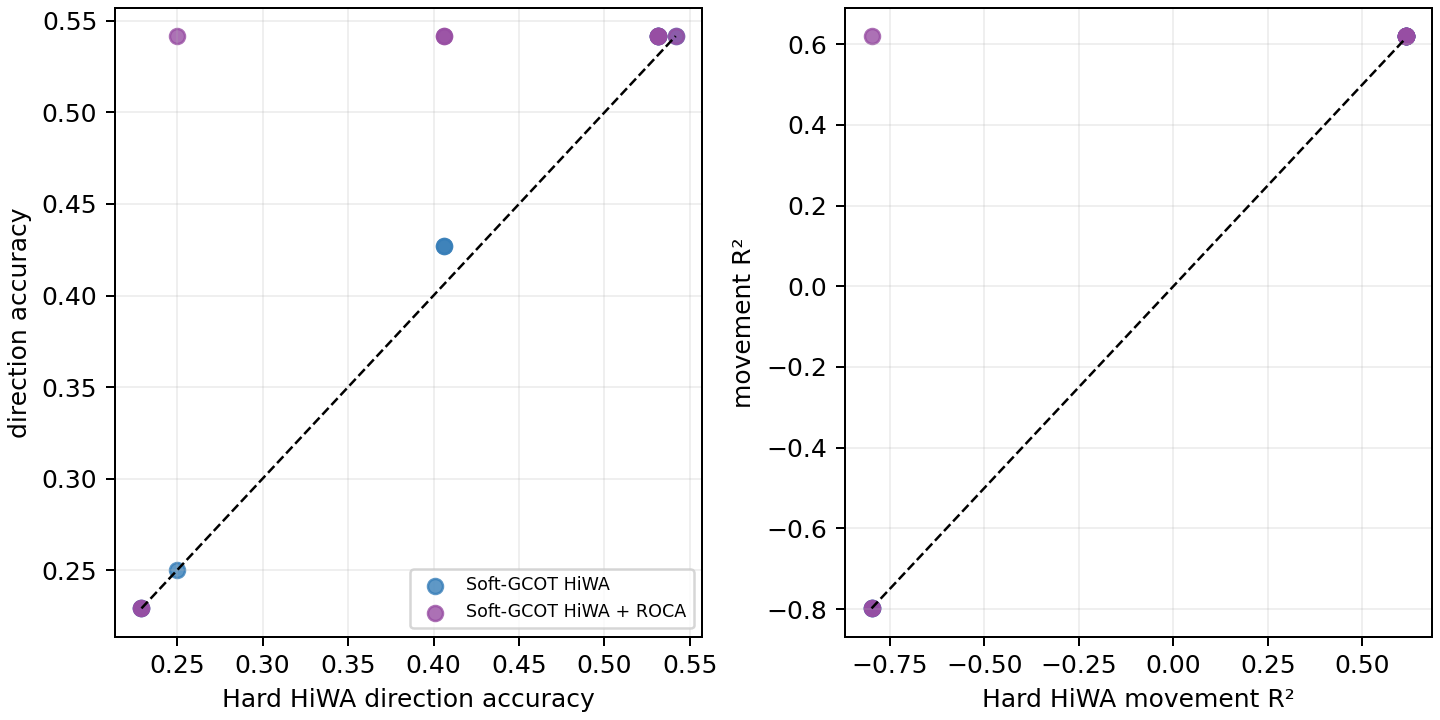
\includegraphics[width=0.83\linewidth]{paired_analysis_full_support_roca_seeds_80_89.png}
\caption{严格 full-support、公平分组协议下的 ROCA 配对结果。每个点对应一个随机 seed；详细数值见表~\ref{tab:main-results}。}
\label{fig:paired}
\end{figure}

\section{实验结果}
\subsection{公平主验证}
主验证固定 seeds 80--89。Hard 标签由最终 soft assignments 的 $\arg\max$ 导出；两个 ROCA 候选均使用 full support；所有方法均要求 global 和 primal ADMM residual 同时达标。三种方法均为 10/10 收敛。

\begin{table}[H]
\centering
\caption{公平、收敛的主结果。}
\label{tab:main-results}
\begin{tabularx}{0.92\linewidth}{lCCX}
\toprule
方法 & direction accuracy & movement $R^2$ & 解释\\
\midrule
Hard HiWA & 0.4188 & 0.1908 & 硬分组基线\\
Soft-GCOT HiWA & 0.4271 & 0.1947 & 小幅平均提升\\
Soft-GCOT HiWA + ROCA & 0.4792 & 0.3364 & 当前协议下平均值最高\\
\bottomrule
\end{tabularx}
\end{table}

Soft-GCOT 相对 Hard 的配对平均变化为 accuracy $+0.0083$（bootstrap 95\% CI 为 $[+0.0042,+0.0135]$），$R^2$ 为 $+0.0039$（CI 为 $[+0.0025,+0.0052]$）。ROCA 相对 Soft-GCOT 的平均变化为 accuracy $+0.0604$（CI 为 $[+0.0083,+0.1271]$），$R^2$ 为 $+0.1456$（CI 为 $[+0.0033,+0.4287]$）。但 accuracy 的中位数变化仅为 $+0.0104$，且 ROCA 在 8/10 个 seed 选中事后 accuracy 更高的分支。故应表述为：ROCA 有平均增益与机制支持，但并非无错 selector。

\subsection{机制验证与负结果}
早期机制实验中，seeds 50--69 有 20/20 次选中高 accuracy 候选；三种单轴翻转、seeds 70--79 的 30 个条件均符合预期 determinant；1600 个合成条件的 determinant recovery 为 0.995。它们支持有向体积机制，但部分实验早于统一 full-support 与收敛协议，故不与主表混合统计。随机初始化软分组、温度扫描、退火和仅用运输目标选择分支均未提供可靠提升。

\section{外部数据与适用边界}
\subsection{Indy--Loco：跨记录日 decoder transfer}
Indy--Loco 是公开猕猴到达运动神经电生理数据。本研究将 `indy\_20160915\_01` 作为源日、`indy\_20160921\_01` 作为目标日；50 ms 分箱、平滑并剔除低发放率 unit 后，分别保留 223 与 220 个神经元。源/目标日神经数据各自标准化并降至 8 维 PCA；用源日 latent state 到二维 cursor velocity 训练 ridge decoder。对齐阶段只提供目标日最早 60\% 的神经 bin，目标速度在最后 40\% 的评估才打开。

\begin{table}[H]
\centering
\caption{Indy--Loco 固定 30 轮 pilot。三个 Soft-GCOT 运行均未收敛。}
\begin{tabular}{ccccc}
\toprule
Seed & source-only $R^2$ & Hard $R^2$ & Soft-GCOT $R^2$ & Soft 收敛？\\
\midrule
701 & -0.1110 & -0.0374 & 0.0176 & 否\\
702 & -0.1110 & -0.1607 & -0.0723 & 否\\
703 & -0.1110 & -0.2848 & 0.1174 & 否\\
\bottomrule
\end{tabular}
\end{table}
三个最终 primal residual 为 4.066、3.442、3.741，远高于阈值 0.1。进一步增加迭代、transport-weighted consensus、加入无标签时序动态、源侧 task anchor 或改用单一全局旋转，均未得到合格 transfer。甚至同 session 的 paired Procrustes oracle 也得到负 $R^2$，说明神经 PCA 与瞬时速度并不满足此处所需的近似正交关系。

\subsection{PBMC Multiome：RNA--ATAC 配对检索}
PBMC 数据含 9,631 个共同细胞的 RNA（$9{,}631\times29{,}095$）与 ATAC（$9{,}631\times107{,}194$）测量。cell ID 和 cell type 在构造中被屏蔽，仅用于最终检索评价。以 2,000 个 RNA 高变基因为共同轴，将 ATAC peaks 聚合成 gene activity（13,793 条 peak--gene 边），在拼接后的矩阵上共同拟合 20 维 PCA 和一个 scaler。96 个确定性细胞、4 组条件下，Hard HiWA 在 63 轮形式收敛，$R@1=0$、$R@5=0.0313$；full-support Soft-GCOT 在 54 轮形式收敛，$R@1=0.0208$、$R@5=0.0417$。随机期望分别为 0.0104 和 0.0521，故没有稳定跨模态检索信号。

\subsection{Paderborn：跨转速轴承故障对齐}
在 Paderborn 轴承数据中，源工况为 1500 rpm、目标工况为 900 rpm。每个振动窗口被转换为 log-FFT 频带特征，并在合并后降至 20 维 PCA。两种诊断表明现有最小设计不适合作为性能比较：同一实体仅改变转速时，未对齐 accuracy 已为 0.9375；不同实体同时改变转速时，Hard 为 0.3333（随机水平），Soft 未收敛。问题在于任务要么无需对齐，要么把实体泛化与工况迁移混淆。后续需要多实体、按实体严格切分的协议。

\section{结论与下一步}
Soft-GCOT 已形成可收敛、可审计的软组 HiWA 基线。ROCA 的贡献不是新的监督信号，而是把 soft representatives 作为跨域有向几何锚点，以无标签方式显式解决 $O(3)$ determinant 分支选择。现有主结果支持平均收益，外部实验则明确了方法不能解决的情况：不收敛的 ADMM、不可正交的跨模态关系和不可识别的任务设计。下一步应在冻结的 full-support、公平分组与收敛门槛下扩展多 seed 主验证，并对高维/不同 $K$ 的有向结构及低置信规则进行独立验证。

\section*{可复现材料}
核心实现与运行器包括：
\begin{itemize}
\item \path{src/cc_hiwa/soft_hiwa.py} 与 \path{src/cc_hiwa/soft_groups.py}；
\item \path{src/hiwa/hiwa.py}；
\item \path{experiments/hiwa/run_taco_faithful_baseline.py}；
\item \path{experiments/roca/run_component_aware.py}。
\end{itemize}
本报告的 Markdown 源、LaTeX 源、关键结果图、主结果 JSON 与相关测试已随代码包交付。

\end{document}
